\documentclass[a4paper, 12pt]{ctexart}
\usepackage[english]{babel}
\usepackage{hyperref}
\usepackage{amsmath}
\usepackage{amssymb}
\usepackage{amsfonts}
\usepackage{amsxtra}
\usepackage{amsthm}
\usepackage{booktabs}

\usepackage{wasysym}
\usepackage{float}
\usepackage{isomath}
\usepackage{mathtools}
\usepackage{txfonts}
\usepackage{upgreek}
\usepackage{graphicx}
\usepackage{enumerate}
\usepackage{tensor}
\usepackage{pifont}
\usepackage{footmisc}
\newtheorem{theorem}{Theorem}[section]
\newtheorem{lemma}[theorem]{Lemma}
\newtheorem{definition}{Definition}
\newtheorem{condition}{Condition}
%\newtheorem{proof}{Proof}

%\theoremstype{remark}
\newtheorem*{remark}{Remark}

\usepackage[colorinlistoftodos]{todonotes}
\usepackage{listings}
\usepackage{color}
\definecolor{codegreen}{rgb}{0,0.6,0}
\definecolor{codegray}{rgb}{0.5,0.5,0.5}
\definecolor{codepurple}{rgb}{0.58,0,0.82}
\definecolor{backcolour}{rgb}{0.95,0.95,0.92}
 
\lstdefinestyle{mystyle}{
    backgroundcolor=\color{backcolour},   
    commentstyle=\color{codegreen},
    keywordstyle=\color{magenta},
    numberstyle=\tiny\color{codegray},
    stringstyle=\color{codepurple},
    basicstyle=\footnotesize,
    breakatwhitespace=false,         
    breaklines=true,                 
    captionpos=b,                    
    keepspaces=true,                 
    numbers=left,                    
    numbersep=5pt,                  
    showspaces=false,                
    showstringspaces=false,
    showtabs=false,                  
    tabsize=2
}
\lstset{style=mystyle}
\begin{document}
\title{分数阶Poisson过程性质及应用的探究}
\author{吴昆\thanks{无58 2015010625}}
\providecommand{\keywords}[1]{\textbf{\textit{Index terms---}} #1}
\date{\today}
\maketitle

\begin{abstract}
推导了分数阶Poisson过程的分裂性和到达时刻的条件分布. 由于到达间隔时间期望为无限大, 使得我们无法很好刻画到达间隔时间的特征, 更导致更新过程或排队论应用中有直接的困难. 我们先利用Fubini定理推导分数阶矩, 以冀一窥其特征. 再将到达间隔时间概率密度进行截尾, 使其矩有限, 并用于排队论. 计算并仿真了M/G/1排队模型的平稳性质. 理论和仿真结果表明了截尾在现实中的可行性, 而且一阶矩和二阶矩表达式简洁, 可以立即应用于更新过程等其它模型.
\textbf{\textit{KeyWords---}} 分数阶Poisson过程, M/G/1排队模型, 更新过程, 截尾, 矩
\end{abstract}


\section{分数阶Poisson过程的基本性质探究}
\subsection{分数阶Poisson过程文献调研评注}
\subsubsection{复合分数阶Poisson过程的矩}
分数阶Poisson过程及复合分数阶Poisson过程在\cite{1}中已经研究得很详尽了. \cite{7}的2.1节及2.2节补充地给出了复数分数阶Poisson过程的概率密度和一阶矩和二阶矩, 且其二阶矩形式相比\cite{1}(27)更为规整.

将\cite{7}复合分数阶Poisson过程的一阶矩二阶矩抄录如下,

记复合分数阶Poisson过程$Y(t)=\Sigma _{i=1}^{N(t)}X_i$, $\{X_i\}$为独立同分布随机变量且与$N(t)$独立.则,

\begin{align}
E(Y(t))&=\frac{\mu t^{\nu}d_1}{\Gamma (\nu +1)} \label{eq:fpPMom1}\\
E(Y^2(t))&=\frac{\mu t^{\nu}d_2}{\Gamma (\nu +1)}+\frac{2(\mu t^{\nu})^2 d_1^2}{\Gamma(2\nu +1)}\label{eq:fpPMom2}
\end{align}

其中,$d_i=E(X_1^i), i=1,2$.

显然标准分数阶Poisson过程是复合分数阶的特例. 特别地, \eqref{eq:fpPMom1}\eqref{eq:fpPMom2}中令$d_1=d_2=1$即得标准分数阶Poisson过程的一阶矩和二阶矩.

值得一提的是, \cite{1}(27)须要对\eqref{eq:fpPMom2}稍作变换得到. \cite{1}(27)形式为,
\begin{equation}
\tag{equation (27) from \cite{1}}
\bar{n_\mu ^2}=\Sigma_{n=0}^\infty n^2 P_\mu (n,t)=\bar{n_\mu}+\bar{n_\mu ^2}\frac{\sqrt{\pi}\Gamma(\mu +1)}{2^{2\mu -1}\Gamma(\mu+\frac{1}{2})}
\end{equation}

变换用到了$\Gamma(z)\Gamma(z+\frac{1}{2})=2^{1-2z}\sqrt{\pi}\Gamma(2z)$.

\subsubsection{最后一次更新距观测点时长U的概率密度}
\cite{4}研究了最后一次更新距观测点时长U的概率密度, 这是更新过程中的一个重要议题, 并且直接导致了更新过程的检视悖论(inspection paradox). 

记观测时刻为$t_1$. 记$f_{U_{n_1}}$为U在观测时刻计数为$n_1$条件下的概率密度,

\begin{equation}
U_{n_1}{:\mathrel{\mathop=}}[T_{n_1}|N_\beta(t_1)=n_1]\tag{equation (18) from \cite{4}}
\end{equation}
\begin{equation}
f_{U_{n_1}}(t)=\frac{f_\tau^{\ast n_1}(t)[1-F_\tau(t_1-t)]dt}{\int_0^{t_1}duf_\tau^{\ast n_1}(u)[1-F_\tau(t_1-u)]}\label{equation (20) from [4]}\tag{equation (20) from \cite{4}}
\end{equation}

$f_\tau (t)$是到达间隔时间概率密度, $F_\tau(t)$为到达间隔时间概率分布.

代入标准Poisson过程$\mu=1$, 此时$f_\tau^{\ast n}(t)=\lambda e^{-\lambda t}\frac{(\lambda)^{n-1}}{(n-1)!}$满足Erlang分布, 推导U的概率密度$f_U(t)$, 不出意外会推得指数分布.  

\begin{theorem}
强度为$\lambda$的标准Poisson过程中, 观测时刻为$t_1$. U的概率密度在$t\in [0^+,t_1]$中的表达式$f_U(t)=\lambda e^{-\lambda(t_1-t)}$.
\end{theorem}
\begin{proof}
代入\eqref{equation (20) from [4]}得到,
\begin{equation}
f_{U_{n_1}}(t)=\frac{nt^{n_1-1}}{t_1^{n_1}}
\end{equation}

进而
\begin{equation}
\begin{split}
f_U(t)&=\Sigma_{n=0}^{\infty}P(N(t_1)=n)\cdot f_{u_n}(t)\\
&=\lambda e^{-\lambda (t_1-t)}
\end{split}
\end{equation}


\end{proof}
\begin{remark}
课上推导检视悖论时, ``标准Poisson过程的$f_U(t)$同样满足指数分布''的性质起初让我们有些难以接受. 但是上面的论述证实了这一点, 从而可以放心大胆地计算. 但这样的``证明''``舍近求远'', 该结论的本质我猜测是由CTRW(Continuous Time Random Walk)模型和标准Poisson所对应的Kolmogorov-Feller方程的时间可逆性得到.

\eqref{equation (20) from [4]}给出的条件概率密度$f_{U_{n_1}}(t)$只适用于$t \in [0^+,t_1]$. 在$t<0$或$t>t_1$时, 显然$f_{U_{n_1}}(t)=0$. 因此, 由于概率密度的积分为1, 完整的$f_{U_{n_1}}(t)$表达式须增加一项$C\delta (t)$. 当然对应地,\eqref{equation (20) from [4]}所示加项要乘以一个时间区间指示函数. 课上讲过, 这个狄拉克函数项导致了检视悖论.
\end{remark}

\subsubsection{事件到达间隔时间$\{\tau _i\}$独立同分布}
分数阶Poisson过程依然满足$\{\tau _i\}$为独立同分布. 这是由CTRW模型和分数阶Poisson对应的Kolmogorov-Feller方程描述的就是这样的计数变化过程, 因此是分数阶Poisson过程的基本特性. 

对于不满足独立增量和平稳增量的分数阶Poisson过程, 这个性质在推导时相当有用.
\subsection{分数阶Poisson过程的非Markov性}
对此有两点讨论. 

\begin{enumerate}[1)]
\item 到达间隔时间概率密度$\psi (t)$不满足指数分布,   因而有记忆. 但到达间隔时间相互独立. 

\item $N(t)$不满足独立增量. 可以把t写成$t=\Sigma _{i=1}^{N(t)} \tau _i +U$,   由于到达间隔时间有记忆,   最后一次到达到t的时长U是导致$N(t)$不满足独立增量的原因. 

\end{enumerate}

\subsection{分数阶Poisson过程到达时间的条件分布}
利用到达间隔时间$\tau _i$相互独立来推导. 到达时刻$T_i$与到达间隔时刻$\{\tau _i\}$满足$T_k =\Sigma _{i=1}^{k} \tau _i$.

下面计算在$N_{\mu}(t)=n$条件下, t时刻前的n个到达时刻为$T_i$的概率. 
\begin{equation}
\begin{split}
&P(T_1=t_1,  T_2=t_2,  \cdots,  T_n=t_n|N_\mu (t)=n)\\
&=\frac{P(T_1=t_1,  T_2=t_2,  \cdots,  T_n=t_n,  T_{n+1}>t)}{P(N_\mu (t)=n)}\\
&=\frac{P(\tau _1=t_1,  \tau _2=t_2-t_1,  \cdots,  \tau _n=t_n - t_{n-1},  \tau _{n+1}>t-t_n)}{P(N_\mu (t)=n)}\\
&= \frac{\prod _{i=1}^{n}\nu \tau _i^{\mu -1}E_{\mu ,  \mu}(-\nu \tau _i ^{\mu})\int _{t-t_n}^{+\infty}\nu \tau _{n+1}^{\mu -1}E_{\mu ,  \mu}(-\nu \tau _{n+1}^{\mu})d\tau _{n+1}}{P(N_\mu (t)=n)}\\
&= \frac{n!\prod _{i=1}^{n} \tau _i^{\mu -1}E_{\mu ,  \mu}(-\nu \tau _i ^{\mu}) \cdot E_{\mu}\left(-\nu (t-t_n)^{\mu}\right)}{(t^{\mu})^n \Sigma _{k=0}^{\infty}\frac{(k+n)!}{k!}\frac{(-\nu t^{\mu})^k}{\Gamma \left(\mu (k+n)+1\right)}}\label{eq:conddist}
\end{split}
\end{equation}


以上分子中的积分运算用到了\cite{1}的结论$\int _{t-t_n}^{+\infty} \psi _{\mu} (\tau)d\tau = E_{\mu}\left(-\nu (t-t_n)^{\mu}\right)$. 

没有有关Mittag-Leffler函数乘积的恒等式,   以上式子无法再被化简. 

\begin{remark}
上式中令$\mu = 1$,   就得到了标准Poisson过程的条件分布. 

$\mu<1$时, ``标准Poisson过程到达时间条件分布符合独立均匀分布的顺序统计量''这样优秀的性质不再适用. 
\end{remark}

除此之外, 在打草稿的过程中,   我们还推出了以下等式:
\begin{equation}
\int _0^{\tau} E_{\mu ,  \mu}(-\nu \tau _i^{\mu})\tau _i^{\mu -1}d\tau _i =\frac{1}{\nu}[1-E_{\mu}(-\nu \tau ^{\mu})]
\end{equation}
 
\subsection{分数阶Poisson过程的和与分裂}
我们知道,   标准Poisson过程的和依然是标准Poisson过程. 标准Poisson过程的分裂依然是标准Poisson过程: 对于标准复合Poisson过程$Y(t)=\sum_{i=1}^{N(t)}X_i$中,   如果$X_i$为二项分布,   那么$Y(t)$可以分解成两个独立的标准Poisson过程$Y_1(t)$和$Y_2(t)$,   他们的强度分别为$\lambda p$ 和$\lambda (1-p)$. 

对于 $\mu <1$ 的分数阶Poisson过程,   我们证明
其和不为分数阶Poisson过程,   但复合分数阶Poisson过程依然满足分裂. 
\begin{theorem}[分数阶Poisson过程的分裂]
对于复合分数$\mu \leq 1$阶Poisson过程$Y(t)=\Sigma _{i=1} ^{N_{\mu}(t)}Y_i$,   其强度为$\nu$,   $\{Y_i\}$为独立同分布的0-1分布$Y_i\sim b(1,   p)$. 则代表$Y_i=1$到来的计数过程$N_{1}(t)$和代表$Y_2=0$到来的计数过程$N_{2}(t)$均为分数$\mu$阶Poisson过程,   强度分别为$\nu p$和$\nu (1-p)$. 
\end{theorem}
\begin{proof}
根据\cite{1}(54),   复合分数阶Poisson过程的母函数
\begin{equation}
J_{\mu}(s,   t)=E_{\mu}\left(\nu t^{\mu}(g(s)-1)\right)
\end{equation}

0-1分布的$g(s)$为
\begin{equation}
g(s)=pe^s+(1-p)
\end{equation}

因此,   $Y(t)$的母函数为
\begin{equation}
J_{\mu}(s,   t)=E_{\mu}\left(\nu t^{\mu}p(e^s-1)\right)
\end{equation}

即$N_{1}(t)$为$\mu$阶,   强度$\nu p$的分数阶Poisson过程. 同理可证$N_{2}(t)$为$\mu$阶,   强度为$\nu (1-p)$的分数阶Poisson过程. 
\end{proof}
\begin{remark}
实际应用中, 满足分裂意味着对分数阶Poisson过程按照0-1分布进行随机采样, 得到的新过程依然是分数阶Poisson过程.

分裂性可以显然地推广至多分类, 即按照固定概率将每个到达事件分为1到n类, 每类事件的到达计数依然满足$\mu$阶Poisson过程, 强度对应为$\nu p_i$.
\end{remark}
\begin{theorem}[分数阶Poisson过程的和]
$\mu <1$的两个分数阶Poisson过程$N_{\mu ,   1}(t),   $$N_{\mu ,   2}(t)$的和$N^{\prime}(t)$不为分数阶Poisson过程(或标准Poisson过程). 
\end{theorem}
\begin{proof}
\begin{equation}
\begin{split}
P(N^{\prime}(t)=n)&=\Sigma _{j=0}^n P_{\mu ,   1}(j,   t)\cdot P_{\mu ,   2}(n-j,   t)\\
&=(\nu t^{\mu})^n \Sigma _{j=0}^n \Sigma _{k=0}^{\infty}\frac {(k+j)!}{j!k!} \frac{(-\nu t^{\mu})^k}{\Gamma \left(\mu (k+j)+1\right)}\Sigma _{k_2 =0}^{\infty}\frac{(k_2 +j)!}{j!k_2 !}\frac{(-\nu t^{\mu})^{k_2}}{\Gamma (\mu \left(k_2 +j\right)+1)}\\
&=\Sigma _{j=0}^{\infty} \Sigma _{k=0}^j \frac {(\nu _1 t^{\mu}(e^{-s}-1))^k}{\Gamma (k\mu +1)}\frac{(\nu _2 t^{\mu}(e^{-s}-1))^{j-k}}{\Gamma \left((j-k)\mu +1\right)} \\
?&= \Sigma _{j=0}^{\infty}\frac{\left(\nu ^{\prime}t^{\mu ^{\prime}}(e^{-s}-1)\right)^j}{\Gamma (j\mu ^{\prime} +1)}
\end{split}
\end{equation}

若$N^{\prime}(t)$为一分数阶Poisson过程,   则最后一个等号成立,   令$t'=t^{\mu}$,   则$t^{\mu}$各阶系数相等,   因此
\begin{align}
\mu^{\prime}&=\mu\\
\Gamma(j\mu +1)&=\Gamma(k\mu +1)\Gamma((j-k)\mu +1)\cdot\alpha ^k,   \text{$\alpha$ 为定值. }
\end{align}

但是, 由于当$k=0$和$k=j$时,   有$\Gamma(j\mu +1)=\Gamma(k\mu +1)\Gamma((j-k)\mu +1)\cdot1$,   因而$\alpha$只能等于1,   这显然是不对的,   因为在$\mu<1$时,   
\begin{equation}
\Gamma(j\mu +1)\not\equiv\Gamma(k\mu +1)\Gamma\left((j-k)\mu +1\right)
\end{equation}
而$\mu =1$时,   上式恒等,   即标准Poisson过程的和依然为标准Poisson过程. 

\end{proof}




可以证明更强的结论:
\begin{theorem}[分数阶Poisson过程到达间隔时间概率密度卷积$\psi ^{\ast 2}(t)$]
两个分数阶Poisson过程求和得到的计数过程,   其到达间隔时间概率密度$\psi ^{\prime} (t)$不再服从分数阶Poisson过程的到达间隔时间分布. 也就是说,   卷积$\psi ^{\ast 2}(t)$不再服从分数阶Poisson过程到达间隔时间$\psi (t)$的分布. 
\end{theorem}
\begin{proof}
我们知道,   对于同时开始的强度为$\lambda _1,  \lambda _2$的两个标准Poisson过程的和,   可以如下计算在t时刻来了第一个事件的概率密度,   
\begin{equation}
\psi ^{\prime}(t) = \lambda _1 e^{-\lambda _1 t} e^{-\lambda _2 t}+\lambda _2 e^{-\lambda _1 t}e^{-\lambda _2 t}=(\lambda _1 +\lambda _2)e^{-(\lambda _1+\lambda _2)t}
\end{equation}

它仍然满足标准Poisson过程,   且该到达的事件属于两个过程的概率分别为$\frac{\lambda _1}{\lambda _1 +\lambda _2}$和$\frac{\lambda _2}{\lambda _1 +\lambda _2}$,  只与强度有关,   而与时刻t无关. 

而对于分数阶Poisson过程,   采取同样的方法计算,   
\begin{equation}
\psi ^{\prime}(t) = \nu _1 t^{\mu -1}E_{\mu ,  \mu}(-\nu _1 t^{\mu})E_{\mu}(-\nu _2 t^{\mu})+\nu _2 t^{\mu -1}E_{\mu ,  \mu}(-\nu _2 t^{\mu})E_{\mu}(-\nu _1 t^{\mu})
\end{equation}

它是否可以写成$\nu ^{\prime} t^{\mu -1}E_{\mu ,  \mu}(-\nu ^{\prime} t^{\mu})$?

考察最简单的情形,   令$\nu _1 =\nu _2$,   由于$E_{\mu ,  \mu}(\cdot)E_{\mu}(\cdot)$无恒等式变成$E_{\mu ,  \mu}(\cdot)$,   故不行. 


可见其不符合分数阶Poisson过程到达间隔时间的形式. 
\end{proof}
\begin{remark}
更有甚者,   该到达的事件属于两个过程的概率含时刻t,   这意味着包含$N_1 (t)$和$N_2 (t)$的状态,   因此无法利用离散Markov链来研究事件到达时刻观测到的两个分数阶Poisson过程的和的状态集合$\{X_i\}$. 
\end{remark}

\subsection{分数阶Poisson过程的相关函数}
\cite{4}研究了更新过程和分数阶Poisson过程的多元分布, 利用$\{\tau _i\}$的独立性, 和\cite{4}(23)的剩余寿命概率密度$f_{Y_{n_1}}(t)$, 可以推导分数阶Poisson过程的相关函数.将$f_{Y_{n_1}}(t)$中的观测时刻$t_1$设为s.

\begin{equation}
\begin{split}
E(N(s)(N(t))&=E(E(n\cdot N(t)|N(s)=n))\\
&=E(n(\int_s^t f_{Y_{n_1},s}(\tau)\cdot(E(N(t-\tau))+n)d\tau+\int_t^{+\infty}f_{Y_{n_1,s}}(\tau)\cdot n d\tau))
\end{split}
\end{equation}

\subsection{过滤分数阶Poisson过程}
由于分数阶Poisson过程的条件分布无法拆分成n个独立同分布的概率密度, 因此无法继续化简.
\begin{equation}
\begin{split}
\phi _{Y(t)}(\omega)=\int_0^t\int_0^{\tau_n}\cdots\int_0^{\tau_2}&(E_{A_k}(\exp(j\omega \Sigma_{k=1}^n h(t,\tau_k,A_k))|N(t)=n,\tau_1,\cdots,\tau_n))\cdot\\
&\frac{n!\prod _{i=1}^{n} \tau _i^{\mu -1}E_{\mu ,  \mu}(-\nu \tau _i ^{\mu}) \cdot E_{\mu}(-\nu (t-t_n)^{\mu})}{(t^{\mu})^n \Sigma _{k=0}^{\infty}\frac{(k+n)!}{k!}\frac{(-\nu t^{\mu})^k}{\Gamma (\mu (k+n)+1)}} d\tau_1\cdots\tau_n
\end{split}
\end{equation}


\section{分数阶Poisson过程的到达间隔时间}
\subsection{到达间隔时间S的矩}

在研究排队论及更新过程中,  要首先分析出到达间隔时间的特征, 通常只关心其一阶矩和二阶矩.   将它们代入相应公式,   即可算出排队论及更新过程的相应性质. 

我们知道,   $\psi (t)$的Laplace变换函数$F(s)=\frac {\nu} {\nu + s^{\mu}}$,   利用公式
\begin{equation}
E(S^n)=(-1)^n\frac{\partial^n}{\partial s^n} F(s)\bigg|_{s=0}
\end{equation}

可以算得
\begin{equation}
E(S)=\frac{\nu}{(\nu+s^\mu)^2}\mu s^{\mu -1}\bigg|_{s=0}=\infty
\end{equation}
\begin{equation}
E(S^2)=\frac{2\nu}{(\nu +s^\mu)^3} \mu^2 s^{2\mu -2}-\frac{\nu}{(\nu+s^mu)^2} \mu(\mu -1)s^{\mu -2 }\bigg|_{s=0}=\infty
\end{equation}

我们还想求$\frac{E(S^2)}{E(S)}$,   
\begin{equation}
\frac {E(S^2)}{E(S)} = \frac{1}{(\frac{1}{\left(\nu + s^\mu\right)} \mu s^{\mu-1} -(\mu -1)s^{-1})\big|_{s=0} }=0
\end{equation}

\subsection{到达间隔时间S分数阶矩的计算}
矩是一个随机过程的重要性质. 由于S的一阶矩和高阶矩为无限大,   计算阶数小于1的期望,   或许为理解其性质带来一些帮助. 

利用Laplace变换进行计算, 要用到来自\cite{15}的结论, 先将该结论及其证明抄录如下:
\begin{lemma}[分数阶矩的Laplace变换求解法]
对于$\alpha>0$,   记\begin{math}F(\theta)= \mathcal{L}\{\psi (t)\}\end{math} 为$\psi (t)$的Laplace变换,   则有S的$s=n-\alpha$阶矩:
$E(S^s)=(-1)^n\frac{1}{\Gamma (\alpha)} \int _0 ^{\infty} F^{(n)}(\theta)\theta ^{\alpha-1} d\theta$
\end{lemma}
\begin{proof}
由Fubini定理,
\begin{equation}
\begin{split}
\int _0^{\infty}F^{(n)}(\theta)\theta ^{\alpha -1}d\theta &= (-1)^n E\left(\int _0^{\infty}X^ne^{-\theta X}\theta ^{\alpha -1}d\theta\right)\\
&=(-1)^nE(S^{n-\alpha})\int _0^{\infty}\theta ^{\alpha -1}e^{-\theta}d\theta
\end{split}
\end{equation}

当$\alpha >0$,等式右边积分收敛.
\end{proof}

我们先试着求$n=1$,$0<s<1$的正分数阶矩.

\begin{equation}
\begin{split}
E(S^s)&=\frac{-1}{\Gamma (\alpha)}\int _0^{\infty} F^{\prime}(\theta)\theta^{\alpha-1}d\theta\\
&=\frac{-1}{\Gamma(\alpha)}\int _0^{\infty}\frac{(-1)\mu\theta^{\mu-1}\nu}{(\nu+\theta^\mu)^2}\theta^{\alpha-1}d\theta\\
&=\frac{\mu}{(\mu+\alpha-1)\Gamma(\alpha)}\int _0^{\infty}\frac{\nu}{(\nu+\theta^\mu)^2}d\theta^{\mu+\alpha-1}
\end{split}
\end{equation}

取$\mu +\alpha -1=\frac{\mu}{k}$, 即$\alpha=1-\frac{k-1}{k}\mu$, $s=\frac{k-1}{k}\mu$.有

\begin{equation}
\begin{split}
E(S^{\frac{k-1}{k}\mu})&=\frac{1}{\Gamma (1-\frac{k-1}{k}\mu)\frac{1}{k}}\int _0^{+\infty}\frac{\nu}{(\nu +u^k)^2}du\\
&=\frac{\nu^{1/k}}{\nu\Gamma(1-\frac{k-1}{k}\nu)\frac{1}{k}}\int _0^{+\infty}\frac{1}{(1 +(\frac{u}{\nu^{1/k}})^k)^2}d\frac{u}{\nu^{1/k}}\\
&=\frac{k}{\nu^{\frac{k-1}{k}}\Gamma(1-\frac{k-1}{k}\mu)}\frac{k-1}{k^2}\pi \csc (\frac{\pi}{k})\\
&=\frac{1}{\nu^{\frac{k-1}{k}}\Gamma(1-\frac{k-1}{k}\mu)}\frac{k-1}{k}\pi \csc (\frac{\pi}{k})
\end{split}
\end{equation}

其中$k>=2 \text{ and } k\in \mathbb{Z^+}$.

此外,   计算负分数$-\frac{\mu}{k}$阶矩,   $k \in \mathbb{Z^+}$. 

令$n=1$,  有
\begin{equation}
\begin{split}
E(S^s)&=(-1)\frac{1}{\Gamma (\alpha)} \int _0 ^{\infty} \theta ^{\alpha-1} d F(\theta)\\
&=(-1) \frac{1}{\Gamma (\alpha)}[\theta ^{\alpha-1} F(\theta)\bigg|^{\infty}_{0} - \int _0 ^{\infty} F(\theta)d \theta ^{\alpha-1}]\\
&= \frac{1}{\Gamma (\alpha)}\int _0 ^{\infty}F(\theta)d\theta ^{\alpha-1} \\
&= \frac{1}{\Gamma (\alpha)}\int _0 ^{\infty}\frac{\nu}{\nu + \theta ^{\mu}}d\theta ^{\alpha-1}
\end{split}
\end{equation}

以上式子在$\alpha<1+\mu$成立. 在$a=1+\mu$时,   $\theta ^\alpha F(\theta)\bigg|_{\theta \rightarrow +\infty}$为非零有限值,   但这在的求解范围之外.


再令$\alpha=\frac{\mu}{k}$,  有,  
\begin{equation}
\begin{split}
E(S^{-\frac{\mu}{k}})&=\frac{\nu ^{\frac{1}{k}}}{\Gamma (\frac {\mu}{k})} \int _0 ^{\infty} \frac{1}{1+(\frac{\theta}{\nu^{\frac{1}{\mu}}} )^{\mu} } d(\frac{\theta}{\nu ^ {\frac{1}{\mu}}})^{\frac{\mu}{k}} \\
&= \frac{\nu ^{\frac{1}{k}}}{\Gamma (\frac {\mu}{k})} \frac{\pi}{k}\csc (\frac{\pi}{k})
\end{split}
\end{equation}

其中$k>=2 \text{ and } k\in \mathbb{Z^+}$. 

$k=1$时, $E(S^{-\mu})=\infty$. 

本节中的推导用到了
\begin{align}
\int _0^{\infty}\frac{1}{(1+u^k)^2}du&=\frac{k-1}{k^2}\pi \csc (\frac{\pi}{k})\\
\int _0 ^{\infty} \frac{1}{1+u^k } du&=\frac{\pi}{k}\csc (\frac{\pi}{k})
\end{align}
\begin{figure}[h]
\centering
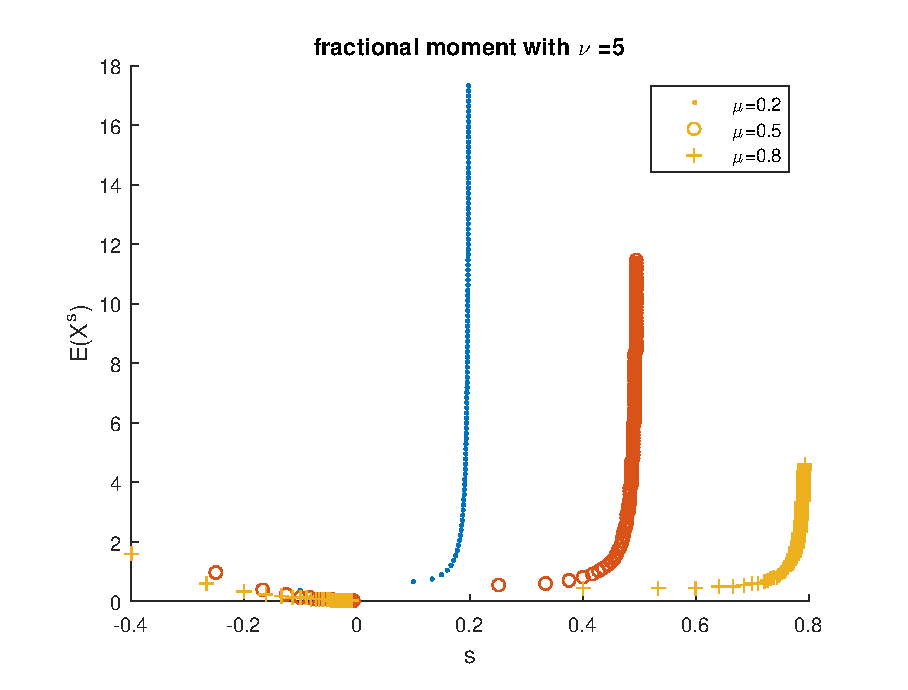
\includegraphics[width=5in]{fractional_moment.eps}
\caption{S的s分数阶矩$E(S^s)$}
\label{fig:1}
\end{figure}
\bigskip

\begin{figure}[h]
\centering
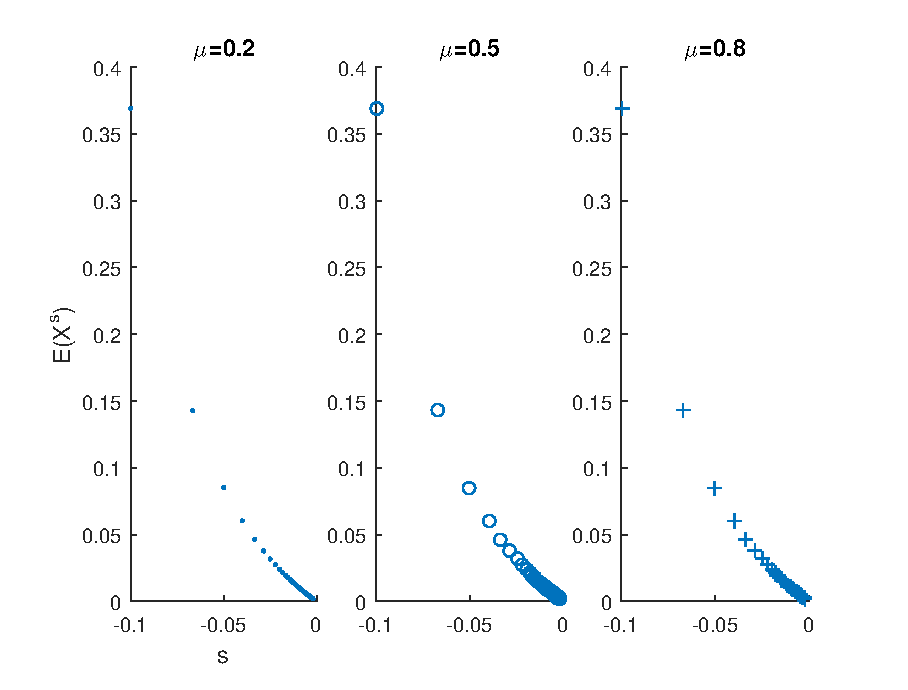
\includegraphics[width=5in,height=3in]{fractional_moment_neg.eps}
\caption{Figure \ref{fig:1}$s\in[-0.1,0]$部分放大}
\label{fig:2}
\end{figure}
\bigskip

由下节的渐进性质, 可知$E(S^s)$在$s\geq\mu$和$s\leq\mu$均为$\infty$, Figure \ref{fig:1}很好地体现了这一点, 正分数阶部分尤为明显.

\subsection{到达间隔时间渐近性质}
\begin{enumerate}
\item 在$E(S)=\infty$时Wald等式依然成立,   可以得到如下渐近性质,
\begin{theorem}
由Wald等式,
\begin{equation}
\lim_{t\rightarrow \infty}\frac{N(t)}{t}=\frac{1}{E(S)}=0,   \text{with probability 1}. 
\end{equation}
\end{theorem}
\item 另一方面   由于$\mu=\infty$,   导致无法运用中心极限定理分析到达间隔时间概率密度$\psi (t)$. 

\item 在\cite{1}中, 给出了在$t\rightarrow 0$和$t\rightarrow \infty$的幂率近似,
\begin{equation}\label{eq:interarrival_approx}
\tag{分数阶Poisson到达间隔时间概率密度幂率近似}
\psi (t) \simeq \begin{cases}
1/\nu t^{\mu +1},  t\rightarrow +\infty \\
\nu t^{\mu -1}, t\rightarrow 0
\end{cases}
\end{equation}
\end{enumerate}

\subsection{对排队论和更新过程的影响}
由于分数阶Poisson过程到达间隔时间一阶矩为无限大,   导致$N_\mu(t)$作为更新过程和以$\Psi(t)$作为G分布的排队模型意义不大. 比如,   对于G/M/1系统,   到来$\lim _{t\rightarrow \infty}\frac{N_a(t)}{t} =0$,   而离开$ \lim _{t\rightarrow \infty} \frac{N_d(t)}{t}=\lambda$,   那么研究稳态情形显然没有什么信息量.

事实上,   \cite{12}\cite{13}\cite{14}等文献研究了到达间隔时间概率密度满足幂率$t\rightarrow +\infty ,  1-\Psi (t)\sim L(t)1/t^{-a} ,  1<a\leq 2$的排队系统,   此时$\psi (t)$一阶矩有限而高阶矩为无限大. 而分数阶Poisson过程的一阶矩也为无限大. 这点可由equation \eqref{eq:interarrival_approx}在$t\rightarrow \infty$的幂率近似直接看出, 相当漂亮.

在这样不利的条件下, 我们能否构造出或者推出一些有意义的模型和结论呢?

\section{M/G/1排队模型与截尾到达间隔时间}
排队模型是电子信息科学中受到广泛应用的模型, 如分析ALOHA, CDMA的信道利用率和碰撞率, 就运用了排队论.
\subsection{M/G/1排队模型}

以顾客为例. M/G/1排队模型是指一条服务线, 顾客的到达间隔时间服从指数分布, 而服务时间符合一般分布G.

如果在顾客离开时刻观测处在排队的人数N,  则N为参数的状态集合$\{N_i\}$满足Markov. 这种分析办法称作嵌入Markov链\cite{16}. 之所以$\{N_i\}$满足Markov性, 是因为顾客到达无记忆. 又由于处在排队的人数N足以描述该系统, 因此就研究$\{N_i\}$.

研究分数阶Poisson过程在M/G/1排队系统中的应用, 由于分数阶Possion的到达间隔时间的一阶矩$E(S)$为无限大, 不满足M/G/1的$\lambda E(S)<1$的要求. 因此须要对G做某种操作.

我们使用一个截尾的服务时间概率密度$\psi ^\prime (t)$(见下一节), 也就是将服务时间限制在$[0,T]$区间内. 它的现实意义是, 当服务时间超过一定时长, 直接放弃转而服务下一个, 这在现实中可以理解为系统死机/放弃消耗时间已超过正常阈值的请求等, 具有现实意义.

本章的工作有两点启示, 其一是使用截尾/超时来处理服务时间概率密度, 解决一阶矩(和二阶矩)为无限大的问题, 其二是含含有$\delta $函数的截尾分布的式子计算.

下一章探讨计算机仿真办法及结果.
\subsection{有关M/G/1系统抄录的式子}
记S为服务时间, 下同.

\cite{10}总结了M/G/1系统的平均性质公式,
\begin{enumerate}[1.]

\item 给定顾客在队列中等待的时间由Pollaczek-Khintchine公式给出,
\begin{equation}
\tag{Pollaczek-Khintchine formula}
W_Q=\frac{\lambda E(S^2)}{2(1-\lambda E(S))}
\label{eq:PK}
\end{equation}

\item 队列中平均顾客数为到达强度$\lambda$与顾客的平均停留时间W乘积,
\begin{equation}
L=\lambda W=\lambda (W_Q+E(S))=\frac{\lambda^2 E(S^2)}{2(1-\lambda E(S))}+\lambda E(S)
\end{equation}

为了使得这些量有限, 须要满足$\lambda E(S)<1$, 即离开率$1/E(S)$小于到达率$\lambda$.

\begin{remark}
$L=\lambda W$用到了Little定理.

上述两个量为到达者观察到的结果.
\end{remark}

\item 引入忙期(系统中至少有一个顾客, 服务线忙)和闲期(系统中没有顾客)概念. 记I和B分别为闲期和忙期的长度, C为一个忙期中服务过的顾客数C.则
\begin{align}
E(I)&=\frac{1}{\lambda}\\
E(B)&=\frac{E(S)}{1-\lambda E(S)}\\
E(C)&=\frac{1}{1-\lambda E(S)}
\end{align}

\end{enumerate}

\cite{16}推导出了M/G/1系统平稳分布(equilibrium distribution)的母函数,
\begin{equation}
\tag{eq:ed}
G_N(z)=\frac{(1-\rho)(1-z)}{S^{\ast}((1-z)\lambda)-z}\cdot S^{\ast}((1-z)\lambda)=\frac{(1-\rho)(1-z)}{1-z/S^\ast((1-z)\lambda)}
\end{equation}

$S^\ast (u)$为服务时间的Laplace变换.

以及逗留时间(sojourn time)和N母函数的关系.
\begin{equation}
G_N(z)=T^\ast ((1-z)\lambda)
\end{equation}

可见, 为了得到M/G/1平稳分布, 以及其他队列的平均性质, 关键是求得G分布对应的服务时间S的一阶矩和二阶矩.

\subsection{截尾到达间隔时间概率密度$\psi _T(t)$与超时率$P_{TD}$}
将分数阶Poisson过程的到达间隔时间概率密度$\psi(t)$在T时刻进行截尾, 得到$\psi _T(t)$, 即令
\begin{equation}
\psi _T(t)=\psi (t)\cdot I(t,0,T) +(1-\int _0^T \psi (t)dt)\delta (t-T)
\end{equation}

其中
\begin{equation}
I(t,0,T)=\begin{cases}
1, 0\leq t\leq T\\
0, \text{otherwise}
\end{cases}
\end{equation}

对应地, 引入超时率$P_{TD}$概念.
\begin{equation}
P_{TD}=1-\int_0^T\psi(t)dt\label{eq:defTD}
\end{equation}
$P_{TD}$表示被截断的概率, 即服务超时未完成而放弃(如丢包, 死机等)的概率.

\subsection{截尾到达间隔时间$S_T$的矩}
先求$\psi _T (t)$的Laplace变换$F_T(s)$.
\begin{equation}
\begin{split}
F _T(s)&=\mathcal{L}\{\psi _T (t)\}\\
&=\int _0^T e^{-s\tau}\psi (t)dt+e^{-sT}(1-\int _0^T \psi (\tau)d\tau)\\
&=\int _0^T e^{-s\tau}d[-E_{\mu}(-\nu \tau ^{\mu})]+e^{-sT}E_{\mu}(-\nu T^{\mu})\\
&=-e^{-s\tau}E_\mu(-\nu\tau^\mu)\bigg|_0^T+\int_0^TE_\mu(-\nu\tau^\mu)de^{-s\tau}+e^{-sT}E_{\mu}(-\nu T^{\mu})\\
&=\int_0^TE_\mu(-\nu\tau^\mu)de^{-s\tau}
\end{split}
\end{equation}

则n阶矩可以如下计算,
\begin{equation}
E(S_T^{n})=(-1)^n\frac{\partial^n}{\partial s^n}F_T(s)\bigg|_{s=0}
\end{equation}

则一阶矩和二阶矩为,
\begin{align}
E(S_T)=&(-1)\frac{\partial}{\partial s}F_T\bigg|_{s=0}
=\int_0^TE_\mu(-\nu\tau^\mu)d\tau  \label{eq:EST}\\
E(S_T^{2})=&\frac{\partial2}{\partial s^2}F^\prime(s)\bigg|_{s=0}
=2\int_0^T\tau E_\mu(-\nu\tau^\mu)d\tau\label{eq:ES2T}
\end{align}

这里用到了$\frac{\partial2}{\partial s^2}e^{-s\tau}=\tau^2e^{-s\tau}$.

\subsection{$E(S_T), E(S_T^2), P_{TD}$随$T$变化图线}

我们作图出不同$\mu$下的一阶矩和二阶矩随T的变化, 作为比较, 同时单独作出了$\mu=1$的情形. 

同时, 作出超时率$P_{TD}\sim T$, $\mu=1$情形只在放大图中出现. 

由于$\mu=1$时矩和超时率上升/下降过快, 覆盖其他图线, 因此作了如上所述的处理.

上述图一律取$\nu=5$.

可以看到,超时率在$T=0$附近有一个陡降. 在$T=5$时, $\mu=0.8$及$\mu=0.5$的超时率已经分别降到了1.29\%和5.03\%, 而$\mu=0.2$也降到了11.17. 在$T=9.4$, $\mu=0.2$的超时率跌破10\%(精度0.1), 到达9.99\%.而此时三者的一阶矩均在1以内. $\mu =0.8$, $\mu=0.5$, 在$T=5$时一阶矩分别为0.4666,0.6756, 即离开强度为2.1432, 1.4808. 对于$\nu=5$来说, 10\%的丢包率和2左右的离开强度尚能接受. 而$\mu=0.2$的情况要相对糟糕一些.  

总的来说, $\mu$越小情况越糟糕. 对于$\mu\geq 0.5$的情况, 截尾的处理办法是可以接受的.



\begin{figure}[H]
\centering
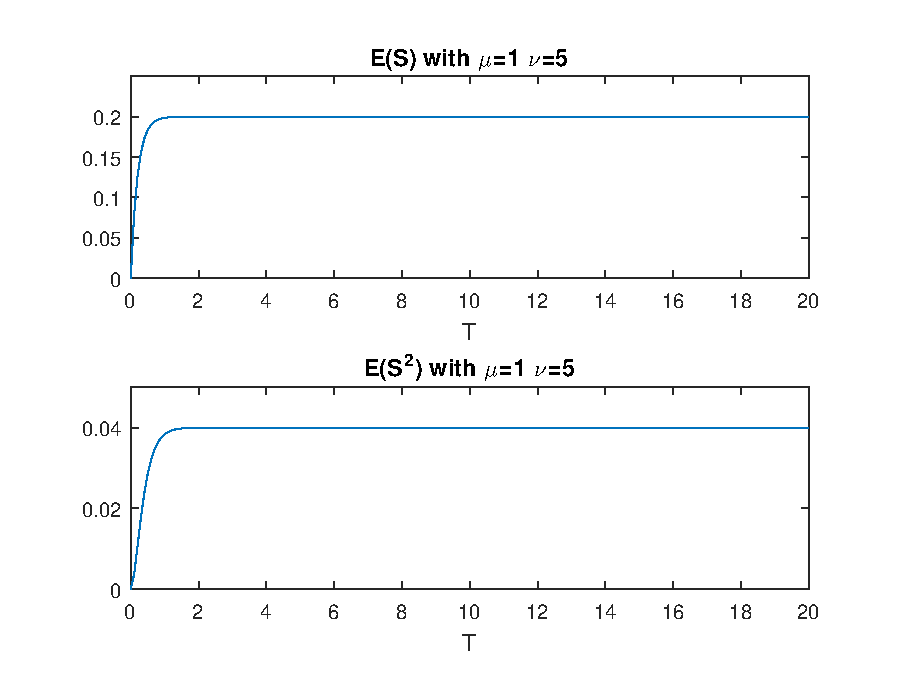
\includegraphics[width=5in,height=3in]{ES_mu_1.eps}
\caption{$\mu =1$时的$E(S_T)$和$E(S^2)$随截尾时刻T的变化}
\label{fig:3}
\end{figure}
\bigskip


\begin{figure}[H]
\centering
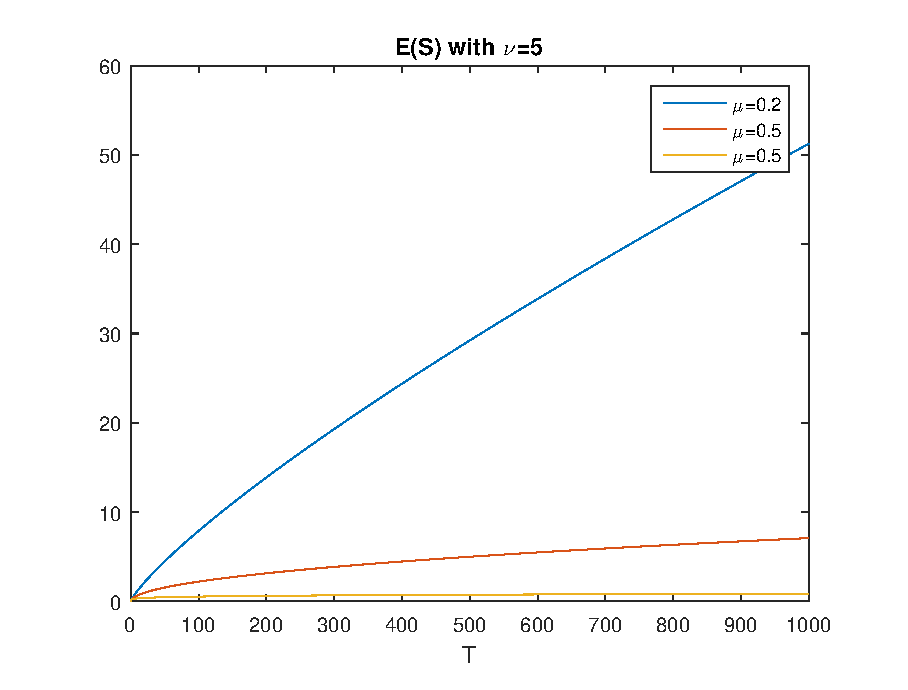
\includegraphics[width=5in,height=3in]{ES.eps}
\caption{不同$\mu$下$E(S_T)$随截尾时刻T的变化}
\label{fig:4}
\end{figure}
\bigskip


\begin{figure}[H]
\centering
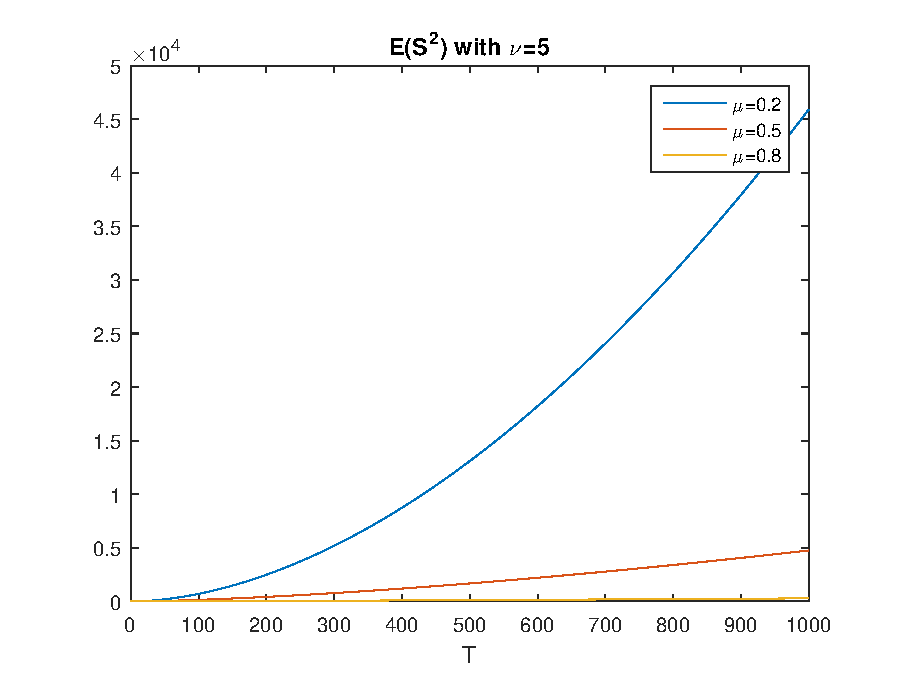
\includegraphics[width=5in,height=3in]{ES2.eps}
\caption{不同$\mu$下$E(S_T^2)$随截尾时刻T的变化}
\label{fig:5}
\end{figure}
\bigskip


\begin{figure}[H]
\centering
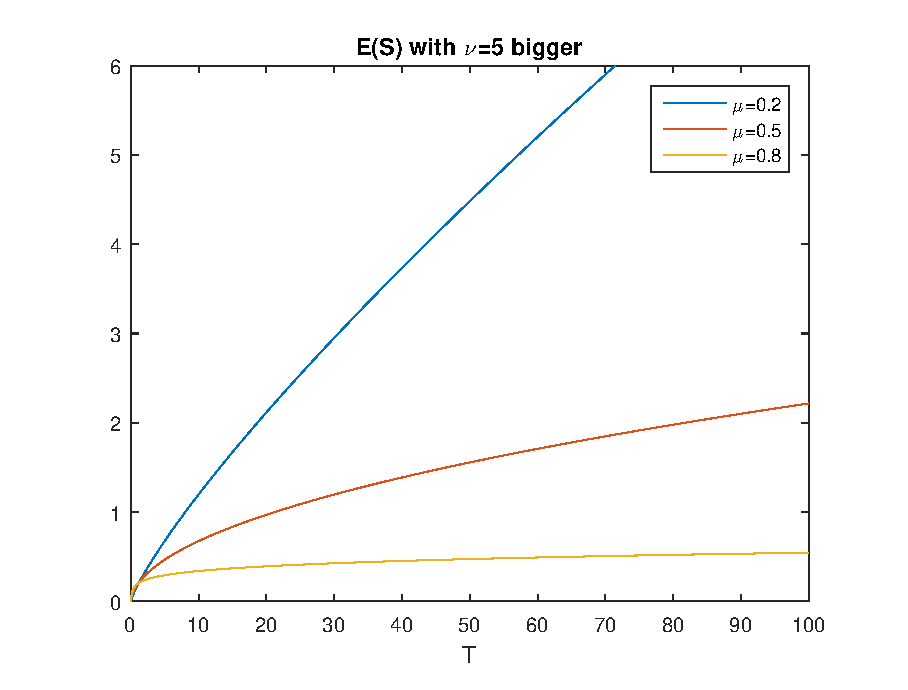
\includegraphics[width=5in,height=3in]{ES_bigger.eps}
\caption{Figure \ref{fig:4} $T \in [0,100]$局部放大}
\label{fig:6}
\end{figure}
\bigskip


\begin{figure}[H]
\centering
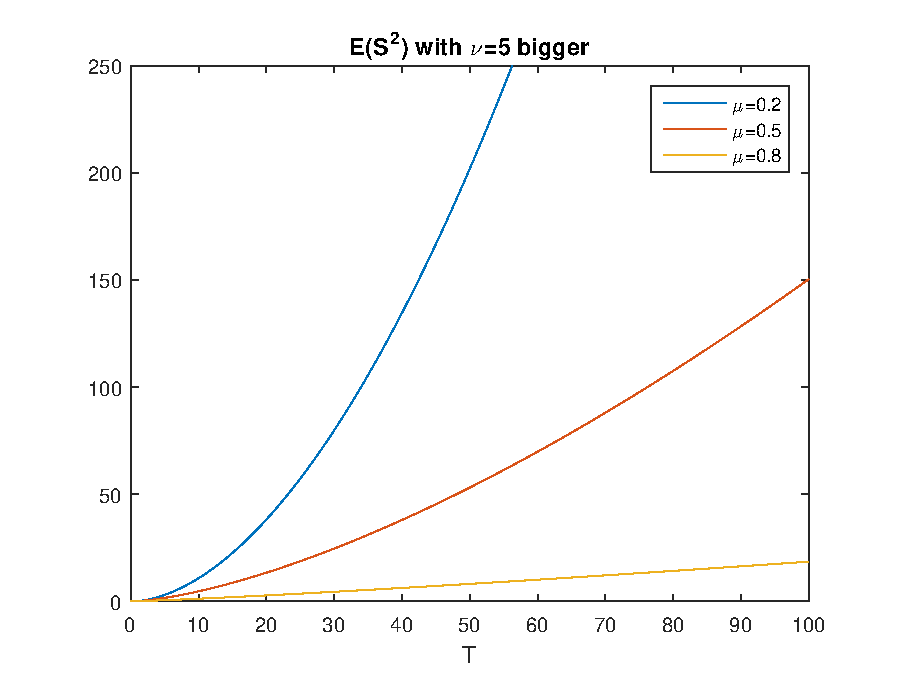
\includegraphics[width=5in,height=3in]{ES2_bigger.eps}
\caption{Figure \ref{fig:5} $T \in [0,100]$局部放大}
\label{fig:7}
\end{figure}
\bigskip

\begin{figure}[H]
\centering
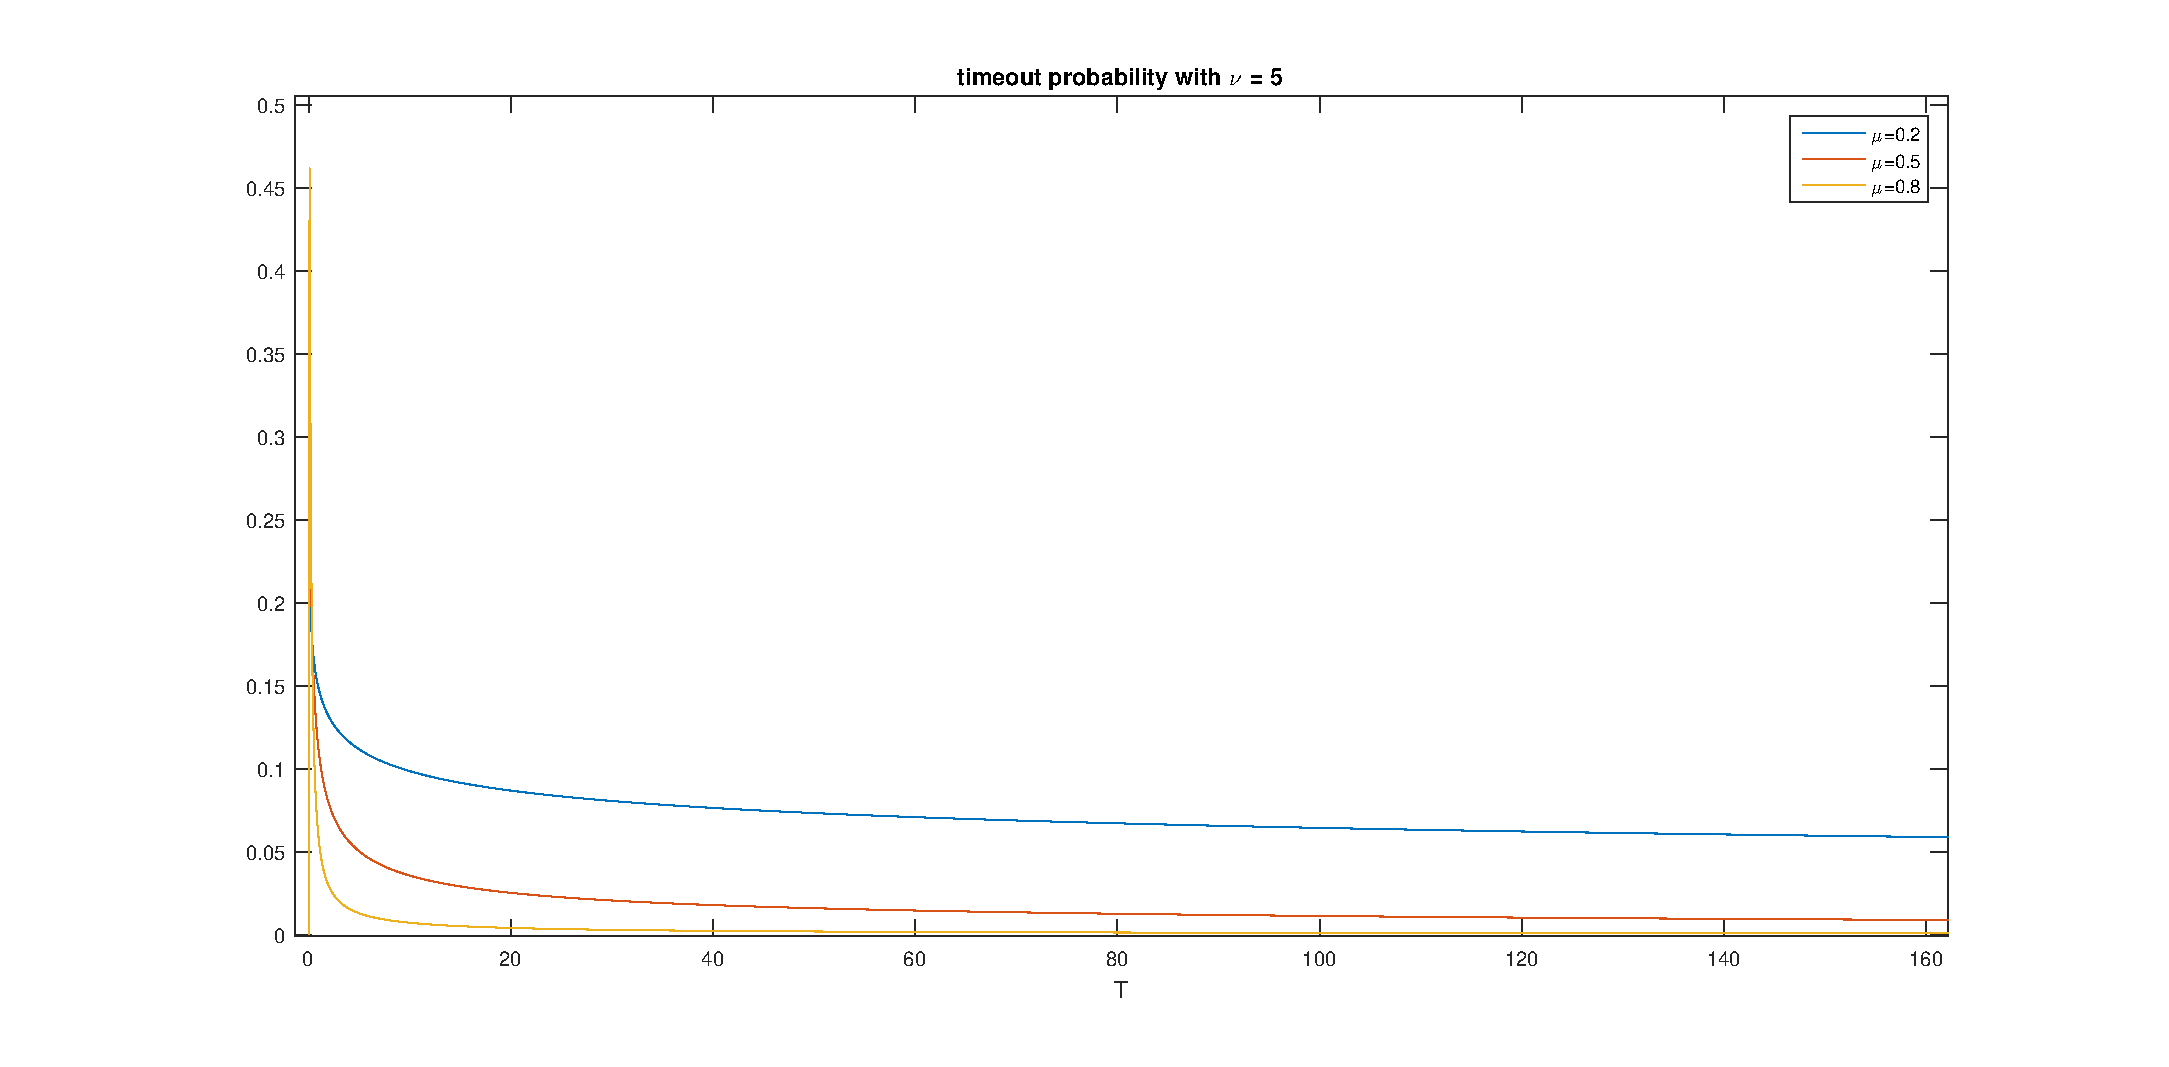
\includegraphics[width=5in,height=3in]{timeout.eps}
\caption{超时率$P_{TD}$随$T$变化}
\label{fig:8}
\end{figure}
\bigskip

\begin{figure}[H]
\centering
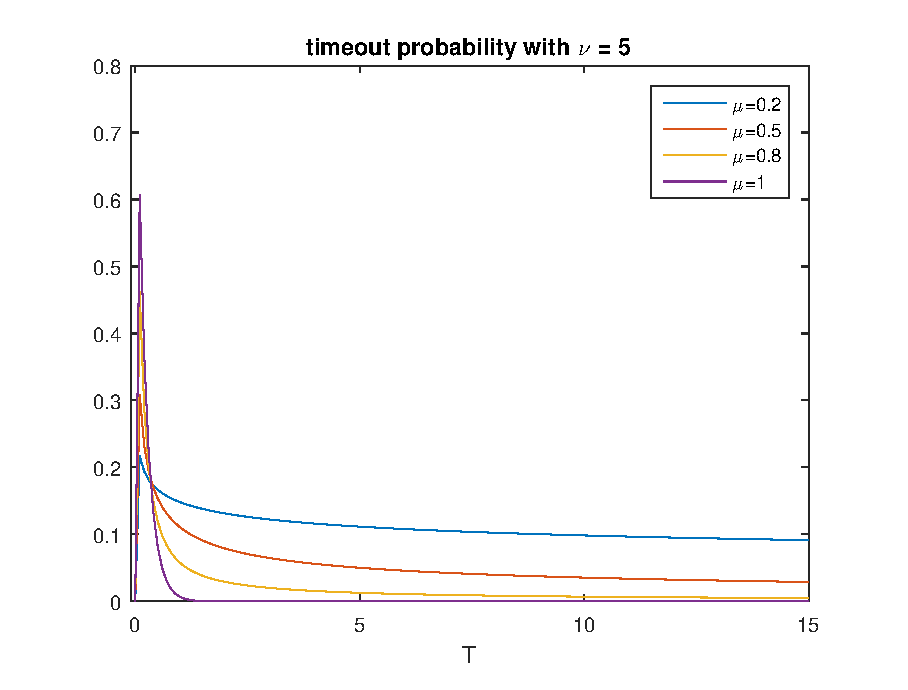
\includegraphics[width=5in,height=3in]{timeout_bigger.eps}
\caption{Figure \ref{fig:8} $T \in [0,16]$局部放大}
\label{fig:9}
\end{figure}
\bigskip

\section{计算机仿真M/$\Psi_T$/1排队模型}
\subsection{截尾服务时间$S_T$随机变量的生成}
使用计算机仿真该排队系统, 第一步准备是生成符合分布的服务时间S随机变量. 在计算机数值系统中, 最基本, 最常见的是均匀分布的随机变量. 因此, 我们要用均匀随机变量, 生成符合分数阶Poisson过程的等待间隔时间概率密度$\psi(t)$的随机变量S. \cite{8}给出了生成方法,

\begin{lemma}[用三个均匀随机变量生成随机变量S]
\begin{equation}
T{:\mathrel{\mathop=}}\frac{|\ln U_1|^{1/\nu}}{\mu ^{1/\nu}}\frac{sin(\nu \pi U_2)[\sin((1-\nu)\pi U_2)]^{1/\nu-1}}{[sin(\pi U_2)]^{1/\nu}||^{1/\nu -1}} \tag{(3.7) from \cite{8}}
\end{equation}

其中, $U_1,U_2,U_3$独立同分布,$X_i\sim U[0,1]$.
\end{lemma}

显然, 把生成的S过一个限幅器即可得到所需的截尾服务时间随机变量$S_T$.

\subsection{排队模型仿真算法}
M/G/1的再生点为顾客服务完离开, 仿真再生点的情形使得仿真算法相当简单. 算法如下,

N为当前系统人数. t为当前时间. ST为随机变量截尾服务时间. ta为随机变量下一个顾客到达所需时间. nc为随机变量服务时间完进入顾客数量.

\begin{lstlisting}[caption=排队系统仿真伪代码]
while 1
    if N==0 %闲置,顾客到来立即开始服务
        以lambda为参数, 生成指数分布随机变量ta;
        T=T+ta;
    else
        随机生成ST;
        N=N-1;
        T=T+S_T;
        以lambda*ST为参数, 生成泊松分布随机变量nc.
        N=N+nc.
\end{lstlisting}

\begin{remark}
这里有一个细节问题须要注意, 当最后一个顾客服务完($t_1$)N=0后在服务时间里没有新的顾客来, 排队系统会闲置, 下一个顾客来($t_2$)系统会立即进行服务. 这种情形需要单独讨论. 算法中处理比较简单, 在顾客服务完条件判断一下生成的随机. 

这会导致构建Markov模型有小小的麻烦, 但是不影响最后平稳分布的结果.
\end{remark}

\subsection{仿真结果}
对$\nu =5$, $\mu=0.5$, T=5时的情形进行仿真. 由\eqref{eq:defTD}\eqref{eq:EST}\eqref{eq:ES2T}计算得到
\begin{table}[!htbp]
\centering
\caption{$\nu =5$, $\mu=0.5$, T=5}\label{tab:lambda2}
\begin{tabular}{cccc}
\toprule
$E(S)$& $E(S^2)$& $1/E(S)$& $P_{TD}$\\
\midrule
0.466637031400487& 0.832431327732974&	2.142993231803241& 0.0503\\
\bottomrule
\end{tabular}
\end{table}

分别取$\lambda=2.0$, $\lambda=2.1$, $\lambda=2.2$, 每次做十遍仿真.

我们发现, 在$\lambda=2.1$和$\lambda=2.0$时仿真结果的超时率和平均队长和理论计算相吻合. 

在$\lambda=2.2$时理论计算$\lambda E(S)>1$, 从Figure \ref{fig:12}中可以直观地看出系统中顾客数量一直在增长, 无法收敛到平稳分布.

\begin{table}[!htbp]
\centering
\caption{$\lambda =2$仿真结果}\label{tab:lambda2}
\begin{tabular}{cccccc}
\toprule
名称& Exp. No.1& 2& 3& 4& 5\\
\midrule
avg Queue Length&
43.5063& 42.1694& 36.2571& 70.6925& 41.6948\\
Timeout Ratio&
0.0506& 0.0501& 0.0497& 0.0510& 0.0501\\
\bottomrule
\toprule
6& 7& 8& 9& 10& 十次平均值\\
\midrule
40.3805& 48.3466& 39.4688& 41.0774& 46.9206& avg45.0514\\
0.0495& 0.0514& 0.0503& 0.0501& 0.0498& avg 0.0502\\
\bottomrule
\end{tabular}
\end{table}

\begin{table}[!htbp]
\centering
\caption{$\lambda =2.1$仿真结果}\label{tab:lambda2}
\begin{tabular}{cccccc}
\toprule
名称& Exp. No.1& 2& 3& 4& 5\\
\midrule
avg Queue Length& 383.1234& 68.2720& 201.3576&  188.3571&  164.2789\\
Timeout Ratio& 0.0515& 0.0478& 0.0506& 0.0503& 0.0509\\
\bottomrule
\toprule
6& 7& 8& 9& 10& 十次平均值\\
\midrule
203.9802& 205.4271&  117.8312&  202.4387&  140.8080&
avg 187.5874\\
0.0510& 0.0506& 0.0493& 0.0494& 0.0498& avg 0.0501\\
\bottomrule
\end{tabular}
\end{table}

\section{结论与展望}
我们首先尝试平行推广标准Poisson过程的结果, 推导出分式Poisson过程具分裂性, 及其到达时刻的条件分布. 由于分数阶Poisson不具备独立增量,平稳增量的性质, 我们能依靠的几乎就是$\{\tau_i\}$独立同分布. 加上结果中的Mittag-Leffler函数, 使得分数阶Poisson不具备``到达时刻的条件分布独立同分布顺序统计量''等等优秀的性质, 从而实际应用中的计算往往不能避免多重积分.

由于更新过程和排队论均极其依赖到达间隔时间的一阶矩和二阶矩, 我们研究了分数阶Poisson过程的一阶矩和二阶矩, 发现均为无限大. 我们利用Fubini定理推导了分数阶矩, 或许可以揭示一部分其性质. 此外还探讨了其渐近性质.

我们将到达间隔时间概率密度截尾, 从而使其一阶矩和二阶矩为有限. 并应用于M/G/1模型. 截尾在现实中有其对应, 且具体数值计算验证了其可行性. 计算机仿真结果验证了理论计算.

对于同样依赖一阶矩和二阶矩的更新过程, 截尾服务时间的一阶矩和二阶矩推导结果可以立即应用, 从而研究其在更新过程的性质. 

截尾的方法或许对研究有同样毛病的分布有借鉴意义.

未来工作有:
\begin{enumerate}
\item 研究Mittag-Leffler函数性质, 及近似表达式. 在近似条件下, 化简结果, 得到分数阶Poisson过程好的性质.

\item 进一步推导M/$\Psi_T$/1排队模型性质, 如根据母函数计算平衡分布等. 并推广至M/G/1排队模型变种.

\item 将截尾服务时间分布应用至更新过程, 推导性质.

\end{enumerate}

\begin{figure}[H]
\centering
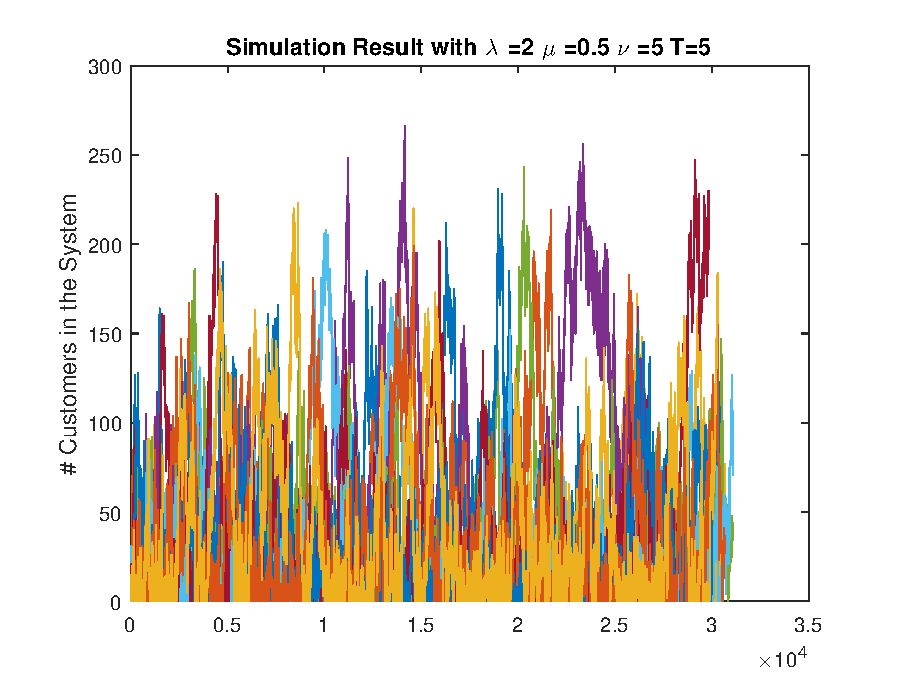
\includegraphics[width=5in,height=3in]{sim.eps}
\caption{$\lambda=2.0$系统中顾客数随时间变化}
\label{fig:10}
\end{figure}
\bigskip

\begin{figure}[H]
\centering
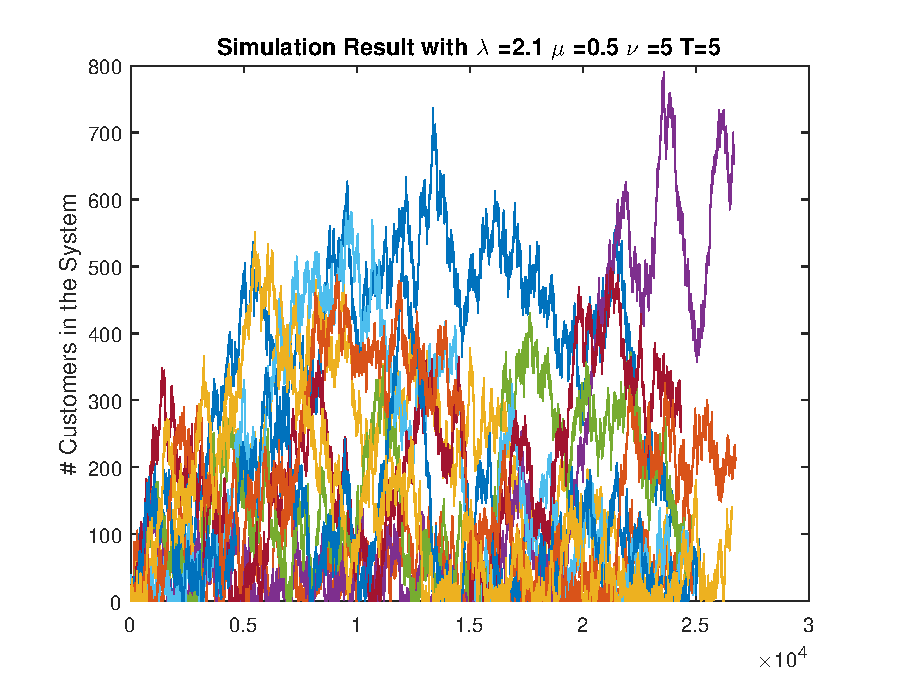
\includegraphics[width=5in,height=3in]{sim21.eps}
\caption{$\lambda=2.1$系统中顾客数随时间变化}
\label{fig:11}
\end{figure}
\bigskip

\begin{figure}[H]
\centering
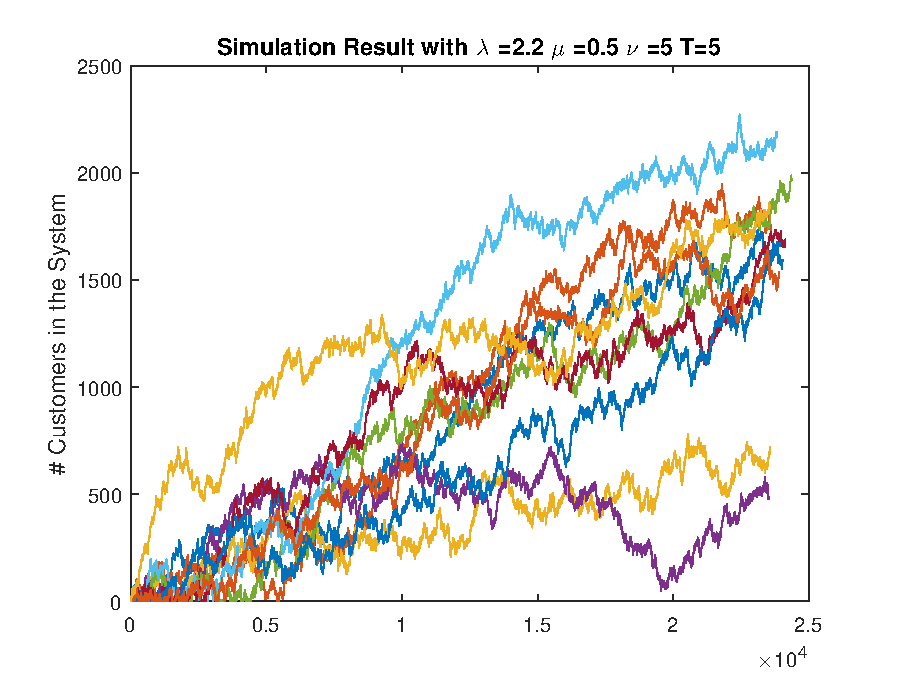
\includegraphics[width=5in,height=3in]{sim22.eps}
\caption{$\lambda=2.2$系统中顾客数随时间变化}
\label{fig:12}
\end{figure}
\bigskip



\newpage
\begin{thebibliography}{1}
\bibitem{1}
Nick Laskin. Fractional Poisson Process[J]. Communications in Nonlinear Science and Numerical Simulation, 8 (2003) 201-213.

\bibitem{2}
Nick Laskin. Some Applications of the Fractional Poisson Probability Distribution[J]. Journal of Mathematical Physics, 2009, 50(11):201-227

\bibitem{3}
Nikolai Leonenko, Enrico Scalas and Mailan Trinh. The Fractional Non-homogeneous Poisson Process[J]. Statistics and Probability Letters, 2016.

\bibitem{4}
Mauro Politi and Taisei Kaizoji. Full Characterization of the Fractional Poisson Process[J]. Europhysics Letters, 2011, 96(2). 

\bibitem{5}
陆大纟金,张灏. 随机过程及其应用[M]. 第2版. 北京:清华大学出版社, 2011.

\bibitem{6}
陆大纟金. 随机过程及其应用[M]. 北京:清华大学出版社, 1984.

\bibitem{7}
王颖. 复合分数阶泊松过程的参数估计及应用[D]. 吉林大学:吉林大学数学研究所, 2015.

\bibitem{8}
Dexter Odchigue. Fractional Poisson Process in terms of Alpha-stable Densities[D]. Case Western Reserve University: Department of Statistics, 2007.

\bibitem{9}
Rudolf Gorenflo and Francesco Mainardi. Laplace-Laplace Analysis of the Fractional Poisson Process[J]. Mathematics, 2013.

\bibitem{10}
Sheldon M. Ross. Introduction to Probability Models[M]. 11th edition. 龚光鲁译. 北京:人民邮电出版社, 2016.

\bibitem{11}
Robert G. Gallager. Stochastic Processes: Theory for Applications[M]. Cambridge University Press, 2014. http://www.rle.mit.edu/rgallager/documents/Renewal.pdf

\bibitem{12}
Mattew Roughan, Darryl Veitch and Michael Rumsewicz. Computing Queue-Length Distributions for Power-Law Queues[J]. Infocom, 1998. 

\bibitem{13}
A. Saichev and D. Sornette. Effects of Diversity and Procrastination in Priority Queuing Theory: the Different Power Law Regimes[J]. Physical Review, 2010, 81(1).

\bibitem{14}
Vladimir N. Zadorozhnyi and Tatiana R. Zakharenkova. Minimization of Packet Loss Probability in Network with Fractal Traffic[J]. ITMM, 2017.

\bibitem{15}
Jeff Schenker. Laplace transform and fractional moments[Z]. https://mathoverflow.net/questions/5525/laplace-transform-and-fractional-moments


\bibitem{16}
J. Virtamo. Queueing Theory: M/G/1-queue[Z]. https://www.netlab.tkk.fi/opetus/s383143/kalvot/E\_mg1jono.pdf
\end{thebibliography}

\end{document}